\documentclass[12pt,a4paper]{article}
\usepackage[utf8]{inputenc}
\usepackage[english]{babel}
\usepackage{amsmath}
\usepackage{amsfonts}
\usepackage{amssymb}
\usepackage{makeidx}
\usepackage{graphicx}
\usepackage{comment}
\usepackage{caption}
\usepackage{subcaption}

\usepackage[left=2cm,right=2cm,top=2cm,bottom=2cm]{geometry}
\title{An outbreak of MRSA at an English hospital}
\author{Alice Ledda, James Price, John Paul and Xavier Didelot}
\begin{document}
\maketitle
\section{The timed tree}
We compute the timed tree using just one sample from each patient. We choose to use the first sample in time for each patient. If there were more than one sequence sampled at the same time we take one at random. As in the previous tree we had to eliminate some samples as they were probably poorly sequenced. These sequences seemed too far away from the others in the tree, placing the most recent common ancestor in the middle ages. The samples we removed are $C00017039$, $C00017244$, $C00021336$, $C00017164$, $C00028623$, $C00021330$, $C00017335$, $C00017158$, $C00017159$, $C00021325$.

The tree is shown in figure \ref{MRSAtree}. The red clades are the ones experimentally classified as MSSA, while the MRSA are shown in black. 

\begin{figure}[hb]
  \centering
  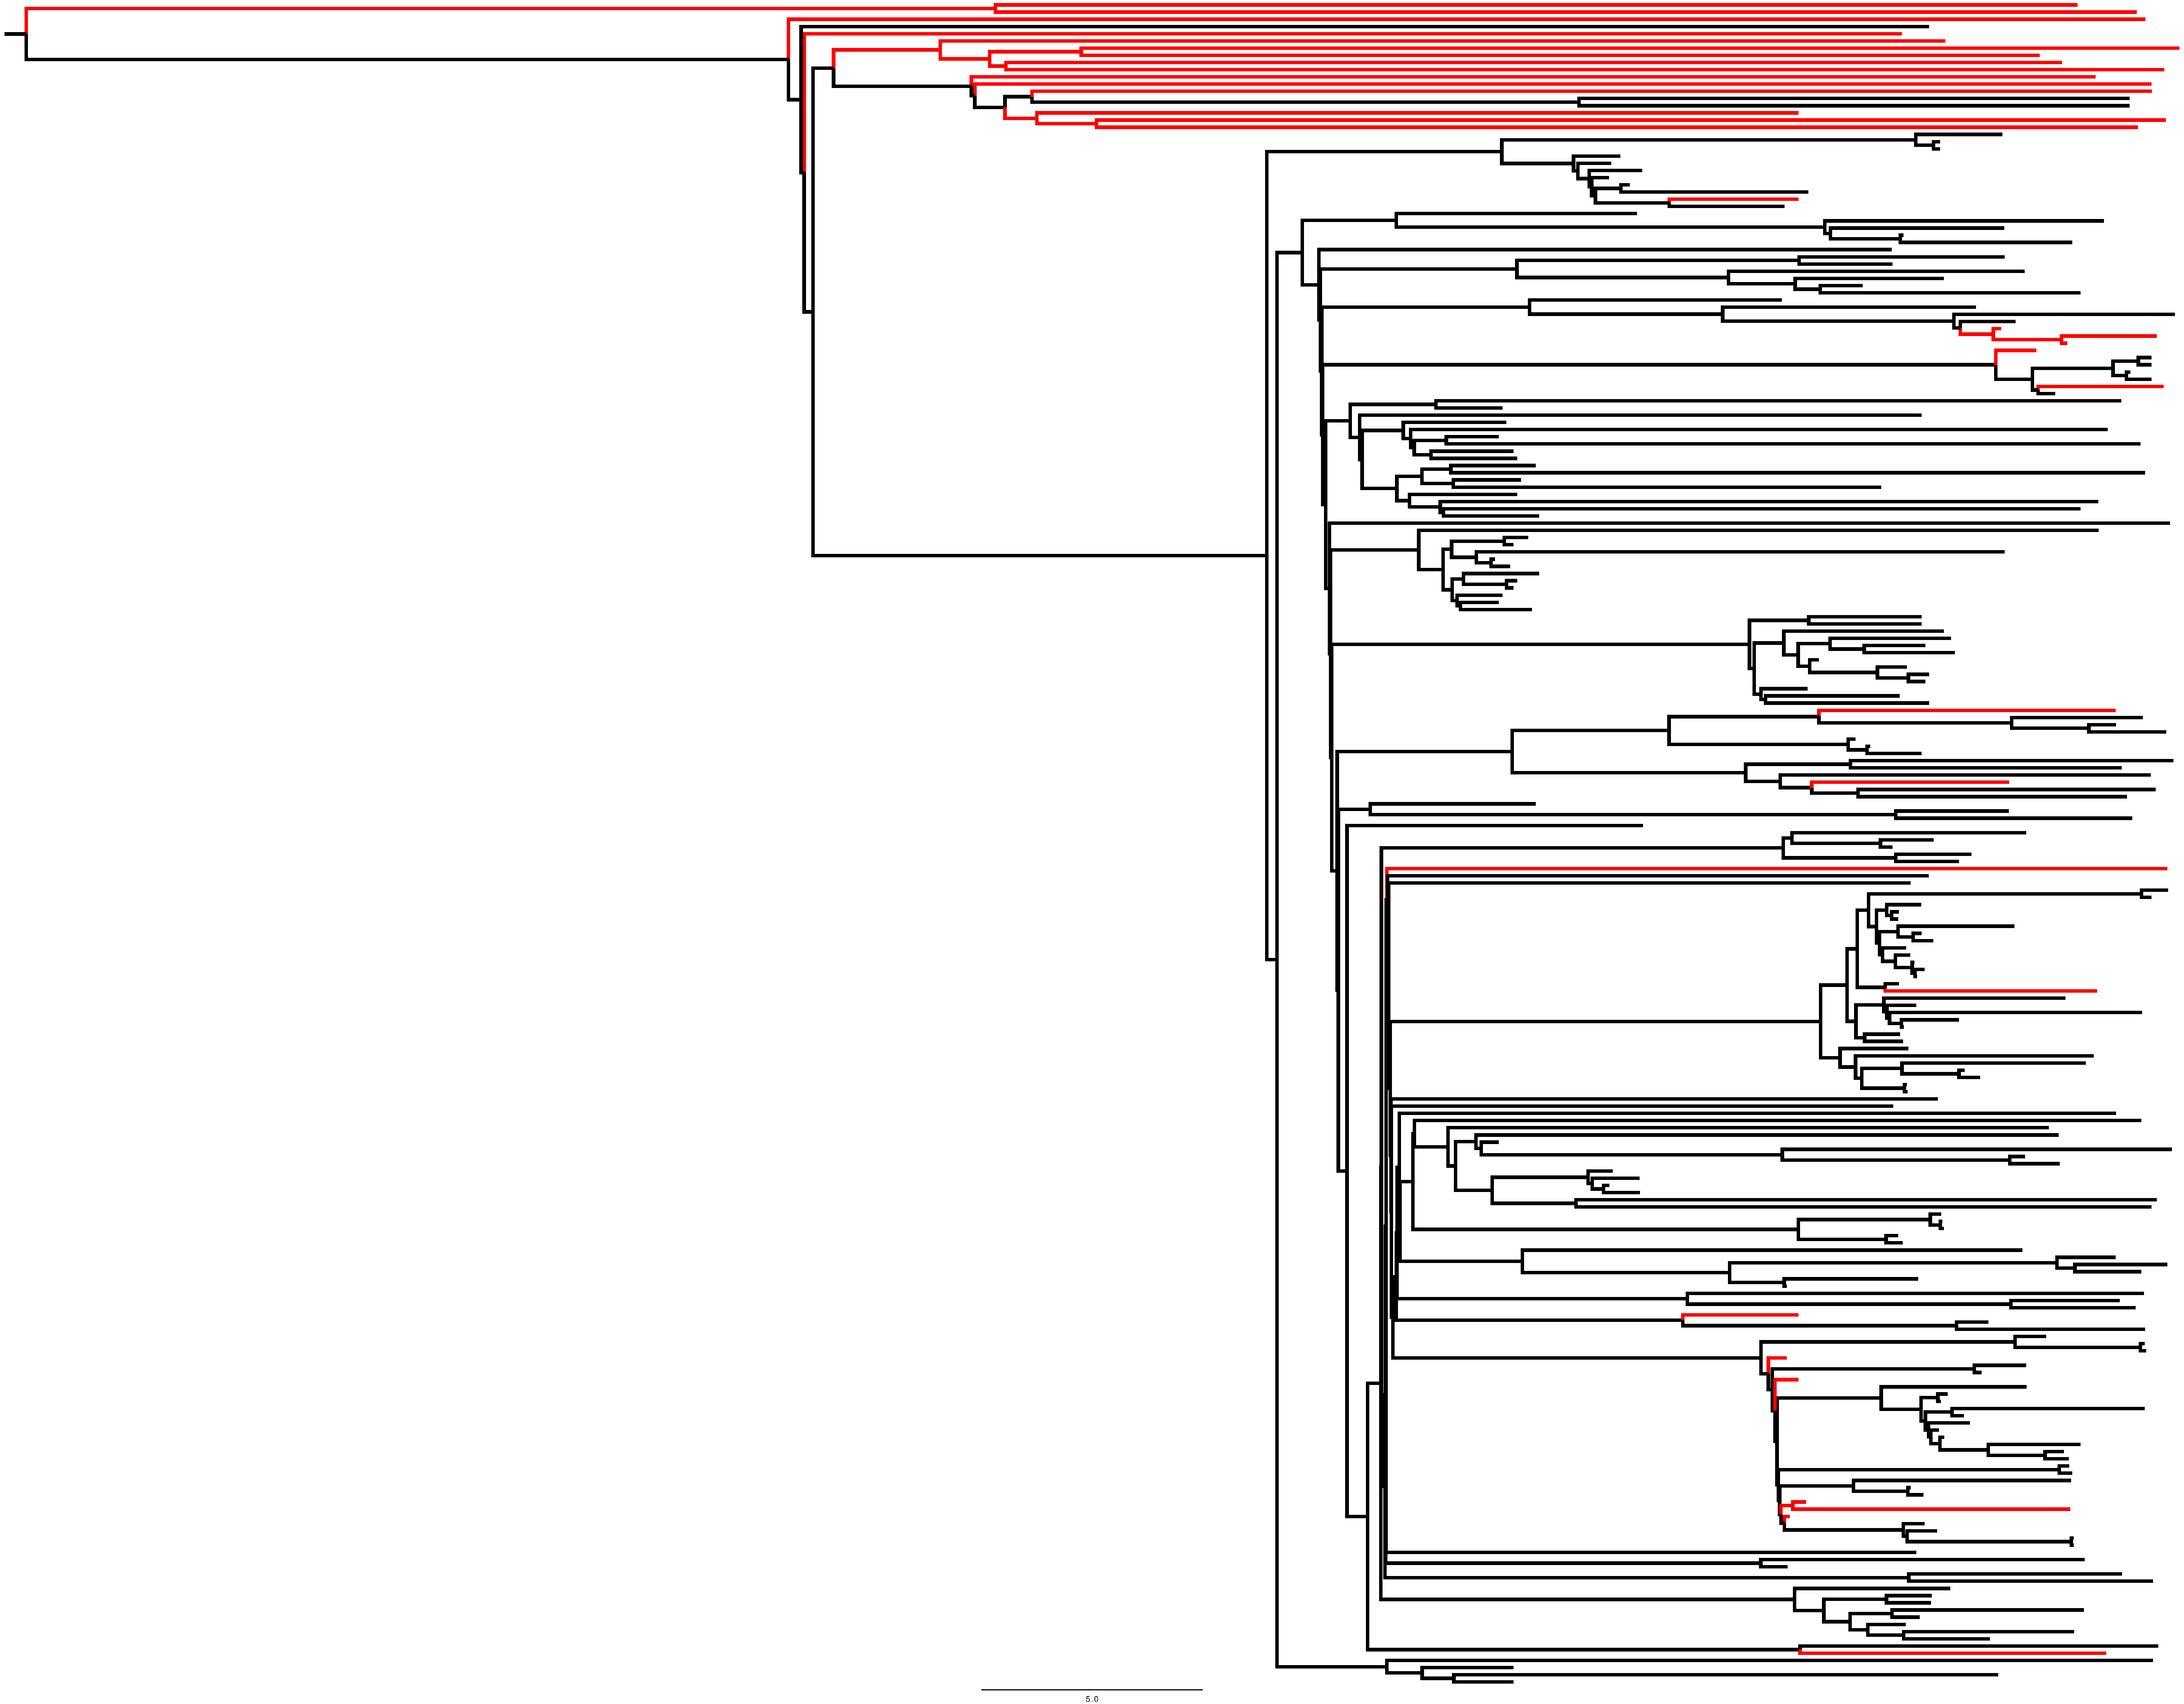
\includegraphics[width=0.8\textwidth]{treeMRSA.pdf}
  \caption[Tree]
   {The timed tree. One sample is present for every sampled individual.The most distant samples have been pruned. In red the samples that were experimentally found MSSA.}\label{MRSAtree}
\end{figure}

As in the previous tree most of the MSSA samples are located in the upper part of the tree, that are the most unrelated samples, yet quite a few of them can be found in the middle part of the tree, sometimes even very related to MRSA samples.

To investigate the MSSA lineages, we retrieved some of the most common genes present in the Staphilococcal Cassette Chromosome \textit{mec}.

\section{\textit{SCCmec}}
The methicillin resistance phenotype in \textit{Staph} is encoded by the \textit{mecA} operon, which is located on a mobile genetic element called \textit{Staphilococcal Chromosomal Cassette mec (SCCmec)}.

To check how the SCCmec was related to the MRSA/MSSA phenotype we looked in the sequences of our sample for the genes that may be present in the cassette. To do so we retrieved the genes that may be present in the cassette and blasted against all our sequences.
The genes that we searched are \textit{ccrA-2, ccrB, ccrC, mecI, mecR1, mecA, IS431, IS272, IS1182},and \textit{Tn4001}. We were not able to retrieve a plausible sequence for the transposase \textit{Tn554}. If we had it we could correctly assign each SCCmec found to the correct class as described in \cite{sscmec}.
 
The sequences used to query blast are reported in fasta format in the github directory created to share with you the files that are too big to be sent by email. You can access it typing 

\verb!https://github.com/aliceLedda/sscmec!

and it should be opened to everybody.
There you can find also a table called  

\verb!cassetteTableAR2.csv! 

in which the presence/absence of the various genes is reported, along with the provenience and the resistance phenotype of the samples.

For each gene we built a contingency table connecting the presence/absence of the gene and the resistance phenotype. We then performed a fisher exact test to determine the association of the gene with the phenotype. The following genes resulted associated with the lowermost possible p-value: \textit{mecI, mecR1, mecA, ccrB} and \textit{ccrA}. We also found a significative association to the phenotype of the insertion sequence \textit{is1272}, both in one or one or more copies, and an association of the insertion sequence \textit{is431}, which is most significative when we test for the presence of 2 copies of it.

All together this evidence tells us that the most common \textit{SCCmec} type in our database is the the type $I$ or type $IV$ of \cite{sscmec} or types $1B$ and $2B$ of the old nomenclature. To distinguish with more precision which one it is we need to have the precise sequences of the $ccrA$ and $ccrB$ genes present in each of the two types. 

The presence of a double copy of the \textit{is431} is incompatible with the presence of the \textit{is1272}, though. So we have to check carefully through the data to see if they most often go together or not. 

%Note that by visual inspection I wouldn't have bet on such an high association between the gene \textit{mecI} and the resistance phenotype as we have 10 case in which we have resistance even if the gene is missing and 4 in which we have the gene and no resistance phenotype.

\textbf{The following samples need to be checked for their Methicilline resistance phenotype:
 \textit{ C00016990, C00017362, C00016980, C00016982} are classified as \textit{MSSA} but they have the \textit{mecA} gene while  \textit{C00017039, C00017330, C00016991, C00017048 } are classified as \textit{MRSA} but I cannot find the \textit{mecA} gene in their sequences.}

Exploring the presence/absence of the cassette as a whole we have three main classes: the samples completely lacking the cassette ($23$ samples), the samples having the complete basic cassette ($mecI, mecR1, mecA, ccrA$ and $ccrB$) ($199$ samples) and a smaller group of just $2$ samples having just a part of the complete cassette, namely $mecR1,mecA$ and $ccrA$. All the samples in this third group is classified as MRSA. There is also a fourth group containing $7$ samples that do not fit in none of the above groups, even if all of them have some of the cassette genes.
To check if any of these groups was associated to a resistance phenotype I did the plot 

 \verb!cassetteRes.pdf!
 
 that you can find in the git folder. Different colour codes are used for the tip names and for the terminal branches. The colour of the tip names represent the resistance phenotype, red being the MSSA, while the colours on the terminal branches are related to the groups described above. In particular in the black terminal branches are the samples having the complete cassette, the red ones are the samples missing the cassette, the blue are the ones with an incomplete cassette and the green are the ones that do not fit in any of the groups.  
 
 
\section{Quinolone resistance}
The quinolone resistance is mainly encoded by point mutations in two housekeeping genes \textit{grlA} and \textit{gyrA}. Yet mutations in the genes \textit{gyrB}, \textit{grlB} and \textit{norA} may be involved in quinolone resistance too \cite{gordon}.

We downloaded a sequence for each of these gene using the references in \cite{gordon} and blasted against the entire database.
Then we retrieved the sequences present in each of the samples and used them to build a tree for each of the two genes.  Both trees (not shown) show that the majority of the samples share the same allele of the gene and only a minority has different alleles, most of them not very different from the most shared one. Each gene has a very different allele, in one case is the C00000890 ($gyrA$), in the other case is C00013995 ($grlA$).

\begin{comment}
\begin{figure}
    
    \begin{subfigure}[b]{0.5\textwidth}
        \includegraphics[width=1\textwidth]{parC.pdf}
        \caption{parC}
        \label{fig:parC}
    \end{subfigure}
    \begin{subfigure}[b]{0.5\textwidth}
        \includegraphics[width=1\textwidth]{gyrA.pdf}
        \caption{gyrA}
        \label{fig:gyrA}
    \end{subfigure}
    \caption{trees for the genes $parC$ and $gyrA$. In both cases, most of the samples have the same allele}\label{fig:Quin}
\end{figure}
\end{comment}


\begin{figure}[hb]
  \centering
  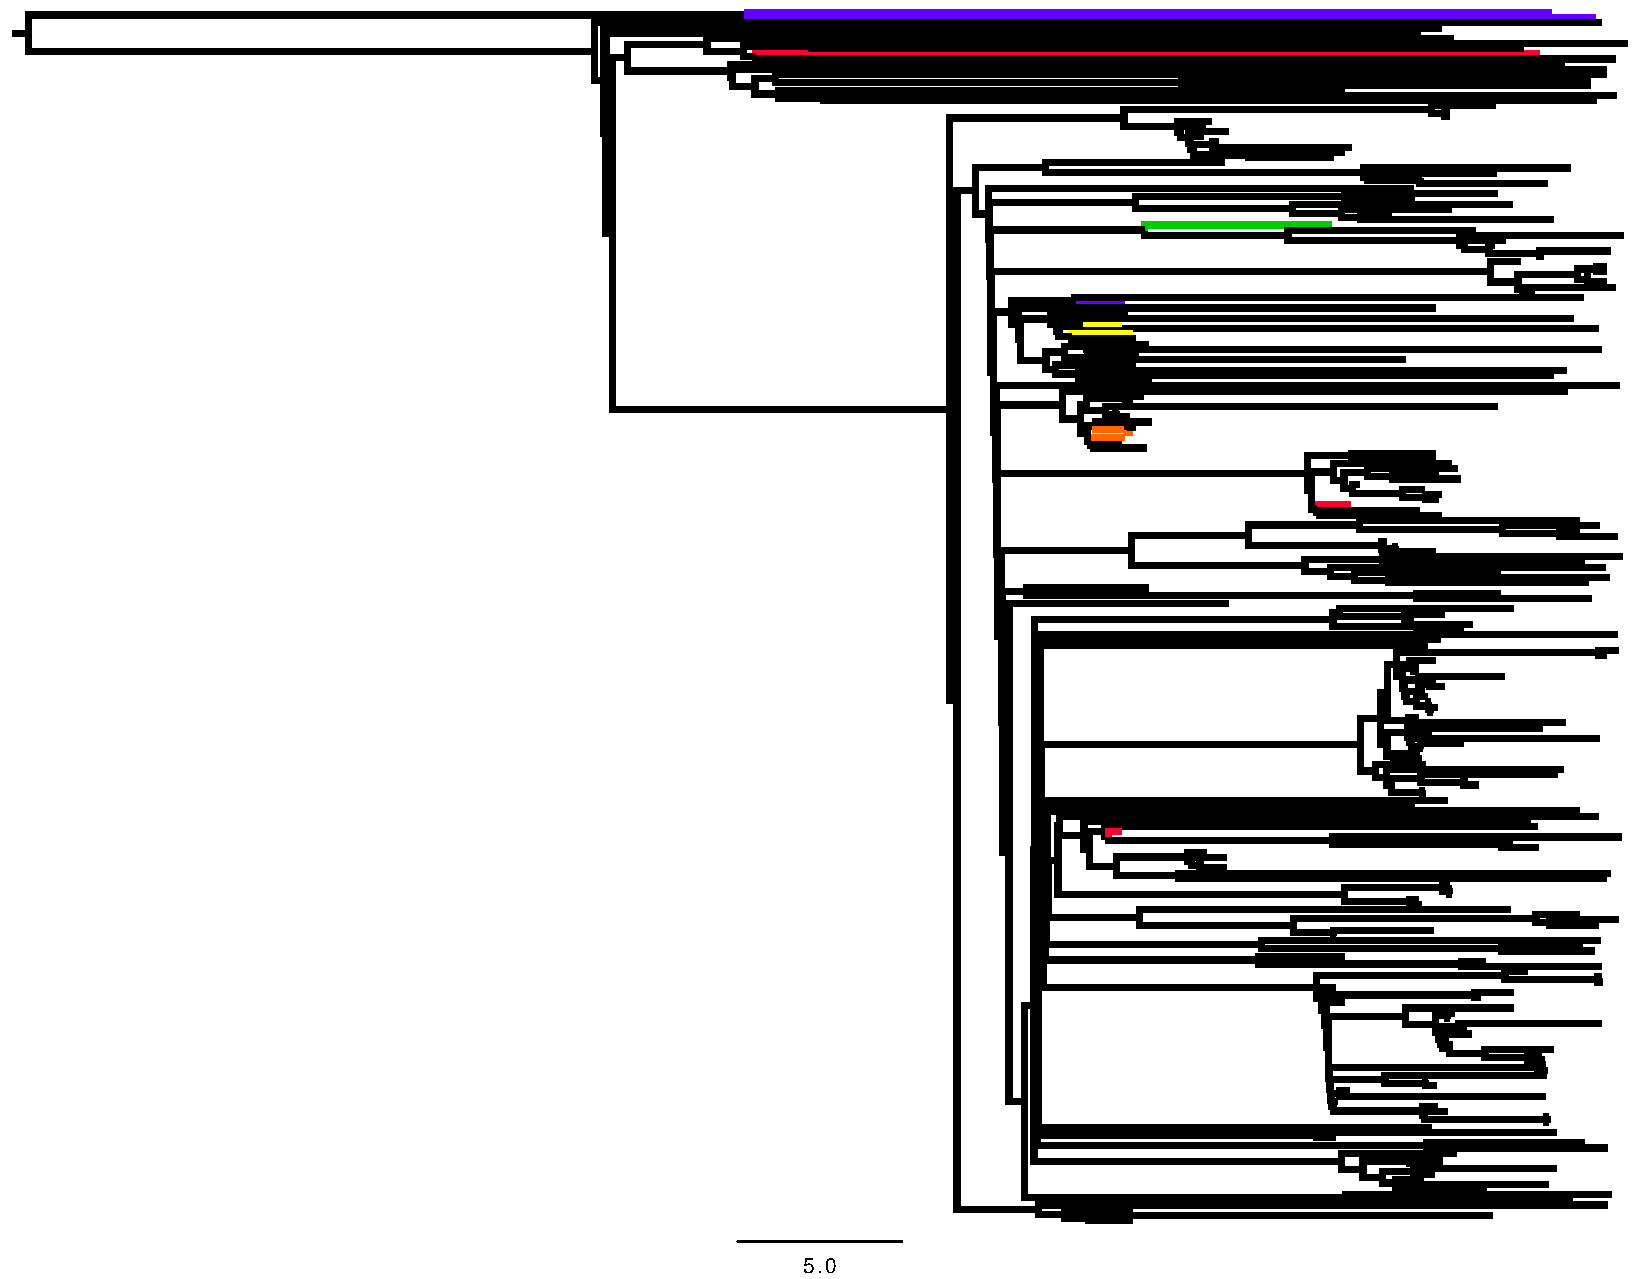
\includegraphics[width=0.8\textwidth]{treeQuin2.pdf}
  \caption[Tree]
   {The quinolone resistance tree. In this tree we show the genotypes related to the quinolone resistance: in black the samples that have the most common genotype of both $gyrA$ and $grlA$, in red the samples that have mutations in the $grlA$ only , in yellow the ones that have mutations in $gyrA$ only, in orange the samples that have mutations in both genes, in blue the samples that have mutations in the $gyrA$ and in one of the other genes and in green the samples that have mutations in $grlA$ and in other genes}\label{QuinTree}
\end{figure}

We reported the mutation pattern displayed from the two genes on the sample tree in figure \ref{QuinTree}. The leaves in black have the most common allele of the 5 studied genes. The leaves in red have a mutated $gyrA$ only, the ones in yellow have a mutated $grlA$ only and the orange in green have mutations in both genes. The ones in blue have mutations in $gyrA$ and in some of the other three genes and those in green have mutations in $grlA$ and one of the other genes.
A resume of the mutated genes long with other useful information about the samples is given in table \ref{tab}. Along with the mutated genes we add information on the patient ID, the origin and the sampling date, the phenotypic characterization of the methicillin resistance and whether or not the sample was included in the Miller et al study \cite{Miller}. The origin of the samples is surely peculiar compared to the entire database shown in figure \ref{fig:from}. All of the mutated samples except one were sampled in Oxford or Brighton. 


%What is striking is that most of the mutated genes, in fact all minus $2$, are in $Staph.$ sampled not recently (before August 07), are MRSA, and are included in the Miller et al study and they come from Oxford. The two more recent ($C00021331$ and $C00017272$) have been sampled more recently ($26/08/2010$ the former and $01/01/2012$ the latter), are not included in the Miller et al study, are MSSA and come from Brighton. Given the distribution of sample's origins shown in \ref{fig:from}, all of this sounds improbable. 
\begin{figure}[hb]
  \centering
  \includegraphics[width=0.5\textwidth]{from.pdf}
  \caption[Tree]
   {The origin of the examined samples as reported in the database.}\label{fig:from}
\end{figure}

\begin{table}[]
\begin{center}
\begin{small}
  \begin{tabular}{ l  c  c  c  c  c  c  c  c  c  c  c }
    
 Sample ID  & Patient  & Origin & Date & MRSA & Study & gyrA & grlA & gyrB & grlB & norA \\ \hline
\hline 
 C00000865  & T162 & Oxford & Jul '97 & MRSA & Miller et al & &\checkmark & & \\ \hline
 C00000890  & T190 & Oxford & Nov '97 & MRSA & Miller et al & \checkmark & \checkmark& & &  \\ \hline
 C00000877 & T173 & Oxford & Jul '97 & MRSA & Miller et al & \checkmark& & & \\ \hline
   C00000901  & T184  & Oxford  & Aug '97 & MRSA & Miller et al & \checkmark & & \checkmark &  \\ \hline
 
  C00000913 & T187 & Oxford & Aug '97 & MRSA & Miller et al & \checkmark & \checkmark & & \\ \hline
  C00000926 & T141 & Oxford  & Nov '97 & MRSA &  Miller et al & & \checkmark & &  \\ \hline
  C00001013 & T156 & Oxford &  Dec '03 & MRSA & Miller et al & & \checkmark & \checkmark & &\\ \hline
  C00001014 & T157 & Oxford & Jul '04 & MRSA &  Miller et al &\checkmark & & \\ \hline
  C00017251 & T249 & Worthing & 17/06/2009 & MRSA & & & & & \checkmark &\\ \hline
  C00017272 & T080 & Brighton & 01/01/2012 & MSSA & &\checkmark & &\checkmark & \\ \hline
  C00021331 & T118 & Brighton & 26/08/2010 & MSSA & &\checkmark & &\checkmark & \\ \hline
  C00021328 & T097 & Brighton & 21/04/2010 & MSSA & &\checkmark & &  \\ \hline
    &  & & & & & & & & \\ \hline
    \hline
  \end{tabular}
  \end{small}
\end{center}

\caption{The table shows the samples that are included in the tree and have mutations in any of the genes associated to quinolone resistance. For each sample is given the sample ID, the patient ID, the origin of the sample and the sampling date, the phenotype for Methicillin resistance and whether they are included in any of the previous studies (\cite{Miller}). A checkmark is displayed when the gene is not the most common allele in the database. }
  \label{tab}
\end{table}

\section{Samples to be re-tested}
The methicillin resistance phenotype should be confirmed for the following samples, as there is discordance between the genotype and the phenotype.
 \textit{ C00016990, C00017362, C00016980, C00016982,C00017039, C00017330, C00016991, C00017048 }
 
 It would also be interesting to know whether the samples that have only a partial \textit{SCCmec} cassette have a different resistance phenotype compared to the others having the entire cassette, or no cassette at all. These are  \textit{ C00017332, C00017299 }
The same for the $7$ samples in the mixed group,  \textit{ C00000844, C00017238, C00018871,C00008959, C00017336, C00017323, C00017330 }.


It would be useful to test the quinolone resistance phenotype of all the samples included in table \ref{tab} along with any other sample included in the table

\verb!cassetteRes.pdf!

\bibliography{bib.bib}{}
\bibliographystyle{plain}

 \end{document}